RGA wird benutzt, um systematisch zu überprüfen, wie SISO ähnlich ein System ist. Das Ziel ist es zu bestimmen ob ein $m \times m$ MIMO-system auch mit einem $m$ SISO-Kontroller eine befriedigende Kreisverstärkung erzielen kann. 
Das RGA ist schlussendlich eine Matrix mit den Verhältnissen aller Übertragungsfunktionen bei einer gegebenen Frequenz $\omega$ 

Die Extremfälle für die Übertragungsfunktion $P_{11}$ werden illustrativ mit folgender Abbildung dargestellt: 
\begin{center}
    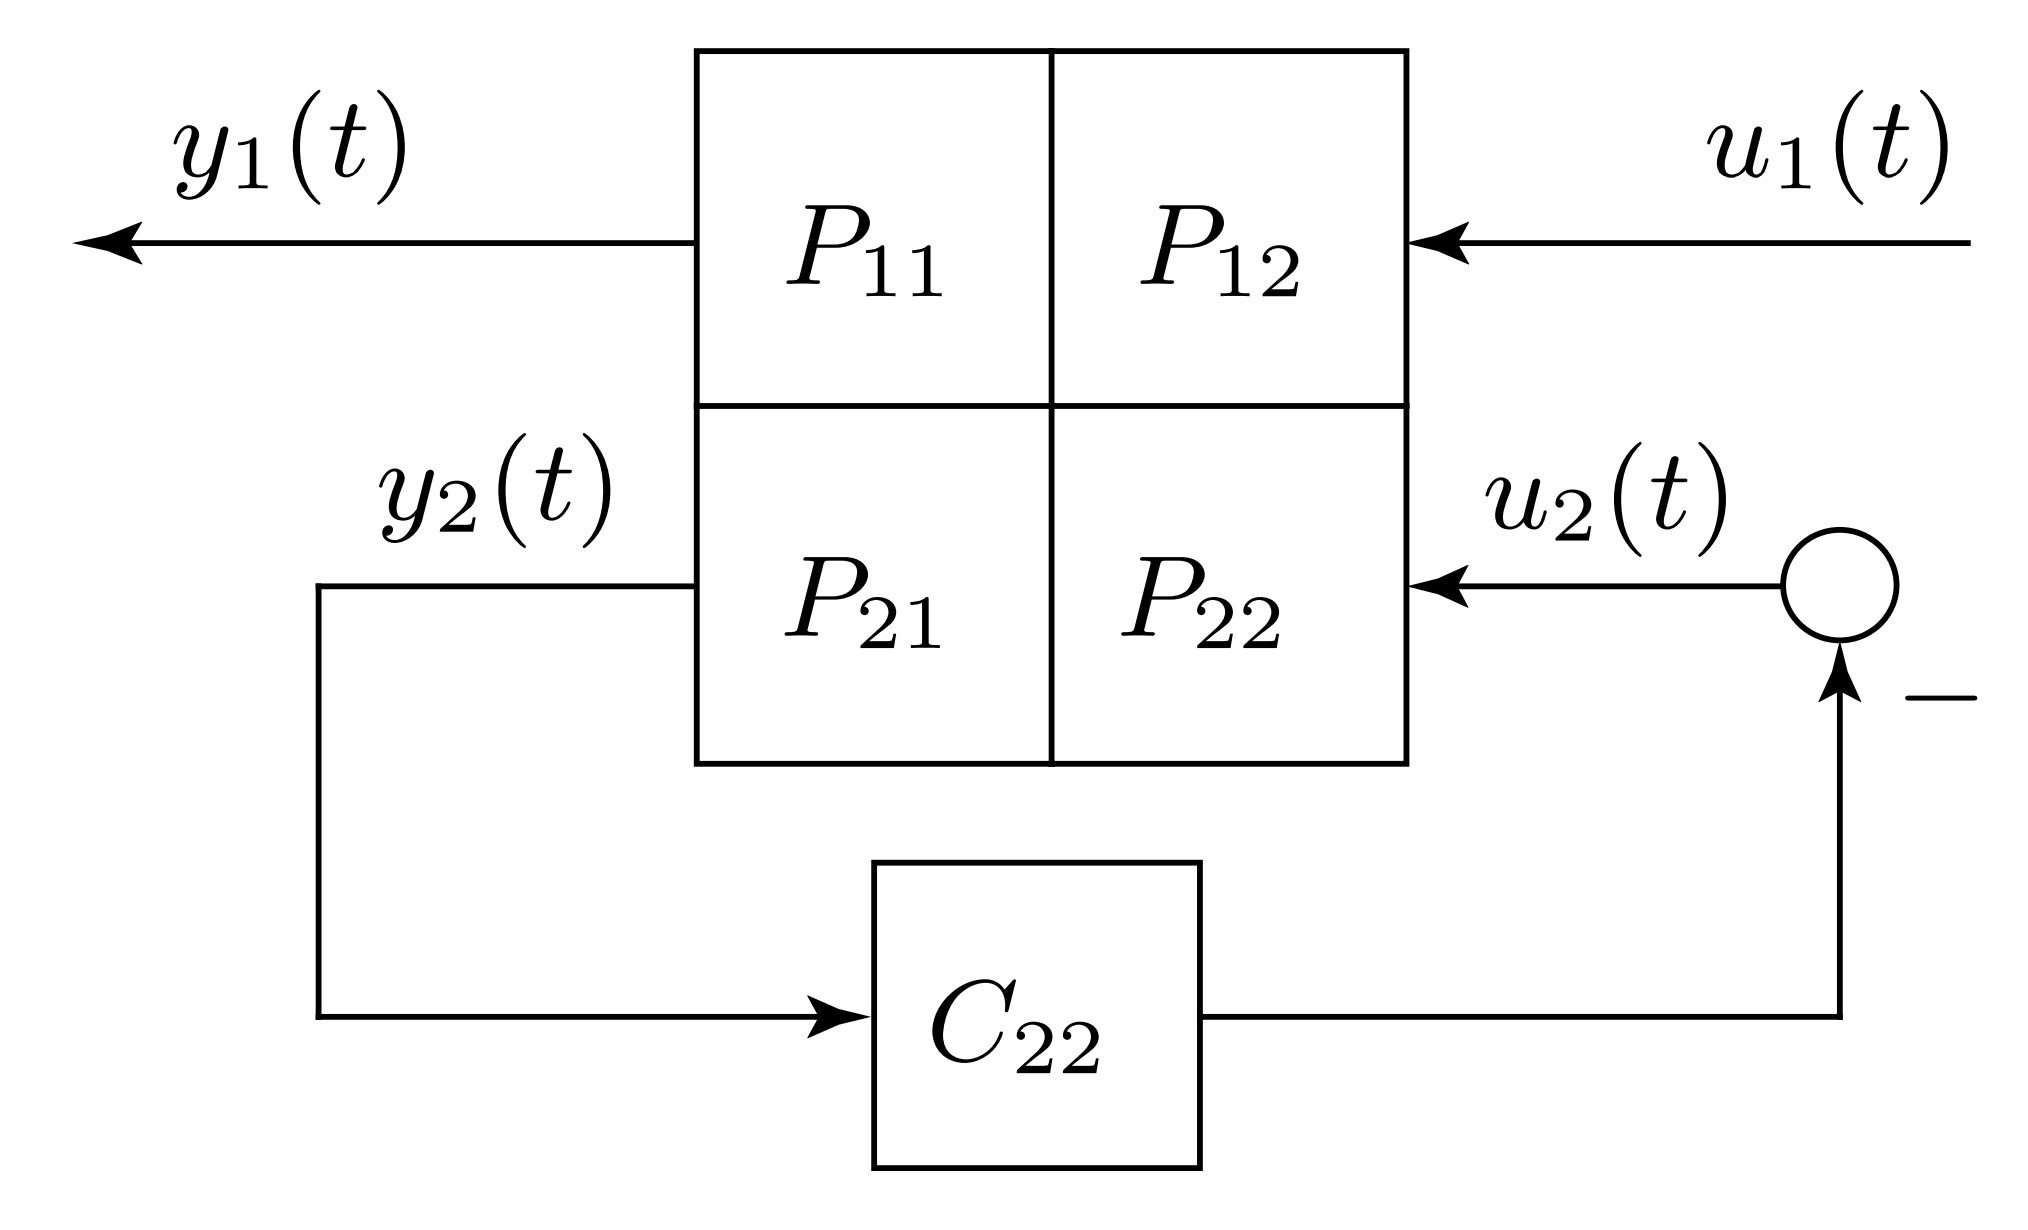
\includegraphics[width = 0.4\linewidth]{images/06/RGA.jpg}
\end{center}
Der Regler $C_{22}$ sollte dabei als eine Art hypothetische Grösse verstanden werden, mit der entweder $u_{2}(t) = 0$ oder $y_2(t)=0$ gesetzt werden kann.

\textbf{Extremfall 1: 'open-loop'} $\boxed{C_{22} = 0}$

Das System wird 'open-loop' betrachtet: Es wird angenommen dass der Regler $C_{22} = 0$ ist, d.h dass nur der Eingang $u_1$ den Ausgang $y_1$ beeinflusst. während im allgemeinen Fall alle anderen Eingänge null sind: $u_j=0 \forall j \setminus \{1\}$
in diesem Fall ist die Übertragungsfunktion von $u_1$ auf $y_1$: 
\[P_{u_1\rightarrow y_1}(s) = P_{11}(s)\]
\textbf{Extremfall 2: 'perfect closed-loop'} $\boxed{C_{22}= \infty}$

Es wird angenommen, dass im allgemeinen Fall alle Ausgänge ausser der betrachtete Ausgang $y_1$ perfekt auf null geregelt werden, d.h. $y_i = 0 \forall i \setminus \{1\}$. Im gegebenen Beispiel heisst das, dass $u_2(t)$ so gewählt ist, dass $y_2(t) = 0 \forall t$. Dies wird schematisch mit einem Regler unendlicher Verstärkung $C_{22} = \infty$ dargestellt. Dann ist die Übertragungsfunktion von $u_1$ auf $y_1$:
\[P_{u_1 \rightarrow y_1}(s) = \frac{P_{11}(s)\cdot P_{22}(s) - P_{12}(s)\cdot P_{21}(s)}{P_{22}}\]
\textbf{Der Relative Gain} ist das resultierende Verhältnis zwischen open-loop und closed-loop Verhalten:\[[\,RGA(s)]\,_{11} = \frac{P_{11}(s)\cdot P_{22}(s)}{P_{11}(s)\cdot P_{22}-P_{12}(s)\cdot P_{21}(s)}\]

Dieses Verhältnis hat eine sehr schöne Interpretation: Es wiederspiegelt die änderung der Verstärkung von Eingang $u_1$ auf Ausgang $y_1$ im Fall , dass alle anderen Regelkreise des MIMO Systems perfekt geschlossen werden. Der Relative Gain beantwortet also die Frage: \textit{Wenn ein Regler vom Eingang $u_1$ auf den Ausgang $y_1$ basierend auf dem open-loop System $P_{11}$ ausgelegt wird, welche veränderten Verhältnisse trifft dieser Regler an, wenn er schlussendlich im geregelten MIMO-System verwendet wird?}

\textbf{SISO-fähiges $P_{i,j}(s)$} $\boxed{[\,RGA(s)]\,_{ij}\approx 1}$  

Die Verstärkung von Eingang $u_j$ auf den Ausgang $y_i$ im MIMO-Sysgem ist identischzu Verstärkung der Übertragungsfunktion $P_{ij}(s)$Basierend auf $P_{ij}(s)$ kann also ein sinnvoller Regler entworfen werden, der den Ausgang $y_i$ mit dem Eingang $u_j$ regelt.

\textbf{Nicht SISO-fähiges $P_{ij}(s)$}$\boxed{[\,RGA(s)]\,_{ij}\approx 0}$  
Die Verstärkung der Übertragungsfunktion $P_{ij}(s)$ ist vernachlässigbar im Vergleich zur resultierenden Verstärkung von Eingang $u_j$ auf Ausgang $y_i$ im MIMO System. Basierend auf $P_{ij}(s)$ kann also \underline{kein} sinnvoller Regler werden der den Ausgang $y_i$ mit dem Eingajng $u_j$ regelt.

\textbf{Instabiles Verhalten für $P_{ij}(s)$} $\boxed{[\,RGA(s)]\,_{ij}<0}$
Das Vorzeichen der Verstärkung der Übertragungsfunktion von $u_j$ auf $y_i$ im MIMO System ist unterschiedlich vom Vorzeichen von $P_{ij}(s)$. D.h. ein SISO-Regler, ausgelegt basierend auf $P_{ij}(s)$, hat wenn er im MIMO-System verwendet wurd, eine entgegengesetzte Wirkung. Der Regler führt also z.B als Reaktion auf einen Sollsprung in $y_i$ dazu, dass die Variable $y_i$ nach unten anstatt nach oben gereglet wird, das MIMO System kann mit diesem Regler also destabilisert werden. 

\textbf{Das RGA} ist die Matrix mit den relativen gains aller Übertragungsfunktionen als Einträgen. 

Das RGA einer $2 \times 2$ Regelstrecke $P(s)$ ist: 
\begin{equation*}
\colorboxed{red}{
RGA(s) = 
{\renewcommand{\arraystretch}{2}
\begin{bmatrix}
\frac{P_{11}P_{22}}{P_{11}P_{22}-P_{12}P_{21}} & \frac{-P_{12}P_{21}}{P_{22}P_{11}-P_{21}P_{12}}\\
\frac{-P_{12}P_{21}}{P_{22}P_{11}-P_{21}P_{12}} & \frac{P_{11}P_{22}}{P_{11}P_{22}-P_{12}P_{21}}
\end{bmatrix}
}
}
\end{equation*}

das RGA eines allgemeinen MIMO-Systems $P(s)$ kann wie folgt berechnet werden: 
\[
\colorboxed{red}{
RGA(s) = P(s).\times P(s)^{-\top}
}
\] wobei $.\times$ eine elementweise Multiplikation beschreibt und $P(s)^{-T}$ die Inverse der Transponierten ist. 

\textbf{Eigenschaften des RGA:} 
\begin{itemize}
    \item Die Summe der Spalten und der Zeilen des RGA ergeben immer 1.
    
    \item Ist das RGA bei einer gegebenen Frequenz $\omega$ ungefähr eine Einheitsmatrix:
    \begin{equation*}
        \big[RGA(\jw)\big]\approx 
        {\renewcommand{\arraystretch}{1.5}
        \begin{bmatrix}
            1&0&0\\
            0&\ddots&0\\
            0&0&1
        \end{bmatrix}
        },
    \end{equation*}
    dann ist das betrachtete MIMO-System bei dieser Frequenz mit individuellen SISO-Reglern regelbar.
\end{itemize}
\textbf{Allgemein:} falls in jeder Zeile/Spalte ein Eintrag sehr nahe bei 1 ist und die anderen nahe bei 0, sind diese Kombinationen von Ein- und Ausgängen gut mit einem SISO-Regler regelbar.

